\documentclass{article} % For LaTeX2e
\usepackage{nips13submit_e,times}
\usepackage{hyperref}
\usepackage{url}
\usepackage{tabularx}
\usepackage{textcomp}
\usepackage{amsmath}
\usepackage{amsfonts}
\usepackage{inconsolata}
\usepackage{setspace}
\usepackage{csquotes}
\usepackage{graphicx}
\usepackage{siunitx}
\usepackage{float}
%\usepackage[section]{placeins}
%\documentstyle[nips13submit_09,times,art10]{article} % For LaTeX 2.09


\title{Looking for Low-proficiency Sentences in ELL Writing}


\author{
Shayne Miel \\
{\fontsize{.28cm}{.1cm}\selectfont \frenchspacing smiel@stanford.edu} \\
}

% The \author macro works with any number of authors. There are two commands
% used to separate the names and addresses of multiple authors: \And and \AND.
%
% Using \And between authors leaves it to \LaTeX{} to determine where to break
% the lines. Using \AND forces a linebreak at that point. So, if \LaTeX{}
% puts 3 of 4 authors names on the first line, and the last on the second
% line, try using \AND instead of \And before the third author name.

\newcommand{\fix}{\marginpar{FIX}}
\newcommand{\new}{\marginpar{NEW}}

\nipsfinalcopy % Uncomment for camera-ready version

\begin{document}


\maketitle

\begin{abstract}
Determining whether an author is writing in their native language (L1) or a
second language (L2) is a problem that lies at the intersection of four
traditional NLP tasks: native language identification, similar language
identification, detecting translationese, and grammatical error correction.
In general, the goal of the language
learner is to improve their proficiency until their writing is indistinguishable
from that of a native speaker. By being able to automatically and reliably
determine whether a section of text looks like L1 or L2 text, areas of writing
that still need improvement can be brought to the learner's attention.
Additionally, the state of the art for correcting grammatical errors involves
using machine translation to translate from errorful text to corrected text\cite{chollampatt}
and there is interesting work being done in generating new training examples
by using machine translation to go
from error-free text to errorful text.\cite{liu} Both approaches could be enhanced by a
system that can tell how close sections of the translation are to an L1 or L2
target.

I present Deep Filter, a convolutional neural network that uses a deep network \textit{as}
the convolution, for determining the probability
that an entire essay was written by an English Language Learner (ELL), using the
document-level label of whether the writer's L1 was English. I then use
the unpooled activations from the convolutional filter to provide insight
into the probability that sections of the text were written by a non-native
writer. The model is able to learn to differentiate native from non-native writing,
and can identify both low-proficiency sections of the essays as well as other
idiosyncracies of non-native English writers.
\end{abstract}

\section{Introduction}

One of the largest challenges for non-native English students is learning to
write in a way that reads like native English writing. This is partly due to their
incomplete knowledge of English grammar, but it is also because of the lack of the
internal language model that native writers build up over many years of reading,
writing, speaking, and hearing the language.

An example of an essay from an ELL student is given here to motivate the sort
of issues I am trying to detect:

\begin{displayquote}
I agree Smoking should be completely banned at the entire restaurant in the
country because smoking is bed for and for everyone is non-smoke. I think that
the people is smoking their must stop because healthy are weak and it will kill
you every time. So you will live out it. Smoking should be completely banned at
all the restaurant in the country. It is good idea because smoking is
disadvantages for everybody. It impossible the restaurant is should not have
smoking anywhere but the restaurant is must have Non- smoking for everywhere.
If the restaurant have Non-smoking I believe most of people will go to hear a
lot because it safety and useful. So the guest will happy and you will see
smile of people eating and drinking in restaurant. Sometime someone want to
smoking so the restaurant is will have the Conner in restaurant for smoking.
Therefore, the restaurant is will have Non-smoking for people don't like smoke
and want to safety and useful for eat and drink so we will help you a lot of
country and many people want to go that here everytime. It is should be
completely banned at all the restaurant in the country.

\end{displayquote}

An automated means of providing feedback on areas of text that appear less
like native English writing would be useful to students learning the language.

Prior work in this area tends to focus on grammatical error detection and correction.
However, focusing on grammar is problematic because the lowest proficiency ELL
writers craft sentences that are either too
jumbled to pick out specific grammar rule violations, or are grammatically correct
but still sound unlike the sort of thing a native English writer would write. In
addition, it is hard to get humans to agree on what grammar errors there are in
any given sentence.\cite{bryant}

This paper takes a different approach by trying to discover the areas of the
writing that look the least like native English writing. I use the L1 status of
the writer to determine whether they are a native English speaker or an ELL student,
and then use that information as a proxy for English proficiency. The paper also
introduces Deep Filter, a convolutional neural network over windows of
character embeddings,
in which the convolutional filter is itself a deep network - a bidirectional
LSTM plus fully connected layer - followed by a pooling layer that generates
the probability that a given essay is from an English language learner. I examine
these probabilties against the ground truth, and also use the information prior
to the pooling layer to get probabilities for areas of the text within the essay.

The experiments in this paper use a large corpus of English student essays,
written by both native
English speakers and ELL students, assembled from many smaller
data sets. Section \ref{data} describes the data collection and cleaning process.
The convolutional network is trained on this corpus to differentiate native
and non-native
writing at the document level, and the unpooled window-level predictions of the
convolution layer are used to detect
within-essay sections of low proficiency.

Section \ref{sim-task} provides examples of similar work with respect to the
task and
section \ref{sim-model} with respect to
the model.
In section \ref{models}, I describe the network in detail as well as several
modifications that were tested. Section \ref{experiments} gives the particulars
of the
experiments, including how the corpus was split into training, development, and
testing splits, the
metric used, and the hyperparamters tested. Finally, section \ref{conclusion}
analyzes the
results and provides some next steps for future research.

\section{Related work}

The task of ELL writing detection has not been studied extensively.
Tomokiyo, et al. attempt this task using a private corpus with a naive Bayes
classifier on word unigrams and bigrams.\cite{tomokiyo}
However, their work focuses on text transcribed from spoken recordings,
rather than writing generated by the ELL writer.

\subsection{Similar tasks} \label{sim-task}

A similar task, native language identification, has received more attention.
Malmasi, et al. established the ETS TOEFL-11 corpus, which has been used by a
number of researchers.\cite{malmasi} Unfortunately for the purposes in this
paper, native English writers don't tend to take the TOEFL and as such are not
represented in this work.

Classifying writing from similar language pairs (for instance, Croatian and Serbian)
is also related to this task, in that native and non-native English could be thought
of as two dialects of the same language. There have been
two shared tasks in 2014 and 2015 where SVMs with word and character features have
done quite well on this task.\cite{goutte} However, the presence of different
words and spellings between even the most similar language pairs makes the
task easier than the one presented in this paper.

Finally, detecting translationese is also quite similar to this work in that
beginning ELL students tend to conceive the structure and content of their essays
in their primary language and then translate it to English when setting it
down in writing. Baroni has studied this problem with SVMs on unigrams,
bigrams, and trigrams of words, lemmas, and part of speech tags.\cite{baroni}

\subsection{Similar models} \label{sim-model}

One of the existing challenges for using RNNs and semantic vectors in general
is figuring out how best to encode long documents. The approach taken in this
paper is to use a bidirectional LSTM with a stacked affine layer as a
convolutional filter over sliding windows of text.
This approach bears some similarities to prior work.

Tang, et al. work with both a CNN and an LSTM to compose word vectors into sentence
vectors, and then compose the sentence vectors into document vectors using a
gated recurrent network.\cite{tang} Yang, et al. use a similar
word-layer/sentence-layer architecture, but also provide an attention mechanism
at each layer to enhance the quality of the output vectors.\cite{yang}
The model in this
paper differs from both of these in that the second level vectors contain
overlapping information, due to the overlapping nature of sliding windows.

In \cite{mikolov}, Mikolov describes a way to generate
document vectors by adding a document token to the context of every word in the
document in what is otherwise a standard word2vec model. While this approach
is better than simply averaging all of the word vectors in the document, it
loses important information about the order of tokens that are crucial to
detecting ungrammatical English.

Collobert, et al. use
a convolutional layer with a max pooling layer to generate window vectors
around each word in a part of speech tagging task.\cite{collobert} This is similar
to the model presented here, except that I use an LSTM \textit{as} the convolution.


\section{Data} \label{data}

\subsection{Data collection}

One of the reasons that there are not many papers applying deep learning to ELL
related problems is the lack of a sufficiently sized corpus. In order to collect
enough data to make use of a deep neural network, I brought together a
number of freely available research corpora, as well as some privately held
data sets provided by \href{http://turnitin.com/}{Turnitin (turnitin.com)}.
All essays were written online by students in
6th-12th grade and early college, responding to particular writing prompts.

Details of all 13 corpora are described in Appendix \ref{app-data} in Tables
\ref{data-table}, \ref{L1s-table}, and \ref{further-info}.

\subsection{Data cleaning}

Collecting data from such a varied set of corpora also presents its own challenges,
however. There are many potential differences between data sets collected under
different conditions and in different years/locations. In order to prevent the
model from learning confounds that are unrelated to the proficiency of the writer,
I cleaned the data as much as I was able to. Some potential confounds that I
attempted to remove by cleaning the data are:
\begin{enumerate}
    \item Encoding differences were removed by converting everything to ASCII and
    restricting the range of characters to lie between \textbackslash x32 (Space)
    and \textbackslash x126 (\texttildelow).
    \item Differences in the way paragraphs were recorded were removed by converting
    any consecutive whitespace to a single space.
    \item Confounds due to learning the topic of the prompts that the essays were
    written to were partially handled by ensuring that the train, development, and
    test splits were essays from non-overlapping subcorpora.
    \item In order to avoid picking up on mentions of the student's country of
    origin, I replaced all country names in the training and development splits
    with the word ``COUNTRY''.
    \item In order to ensure that each essay had enough characters to support
    the 100-character convolution described in Section \ref{models}, I removed
    any essay with less than $150$ or more than $4000$ characters.
\end{enumerate}

After cleaning, 77,046 essays remained, split evenly between native English
writers and writers from 24 other native languages.

\subsection{Data splits} \label{Data splits}

In order to ensure that the model is not just learning something about the prompts
that the essays were written to or a quirk of the data set that the essay came
from, I split the training, development, and testing
sets so that each split contains essays from completely different data sets.
The most convincing
argument for the success of this classifier would come from a data set where
there are both native English
and ELL essays written to the same prompt or prompts. Fortunately, the ICNALE,
MOECS, and CEEAUS data sets fulfill this criteria, so they form the test set.

For the development set, I wanted to use essays written to a large number of prompts
without sacrificing too much of the available training data. The FCE data set has
$44$ prompts, so I used it for the ELL essays and an equivalent number of essays
from the ASAP data set for the native English essays. The rest of the data sets
were used for training. Statistics about the splits can be seen in Table
\ref{splits-table}.

\begin{table}[t]
\caption{Corpus statistics for training, development, and test splits}
\label{splits-table}
\begin{center}
\begin{tabular}{l r r r}
\multicolumn{1}{l}{\bf SPLIT} &\multicolumn{1}{r}{\bf $n$ ESSAYS} &\multicolumn{1}{r}{\bf $n$ PROMPTS} &\multicolumn{1}{r}{\bf \% ELL}
\\ \hline \\
Training &  66677  & 95 & 49\%\\
Development & 4236 & 52 & 41\%\\
Testing & 6133 & 3 & 90\%\\
\end{tabular}
\end{center}
\end{table}

\section{Models} \label{models}

There are unfortunately no labels about the proficiency of the essays, much less
subsections of the essays, in the corpus I collected. Instead, I use whether the
writer was an ELL student as a proxy for proficiency. It is not always true that
the ELL essays in this corpus appear to be less proficient than their native
writer counterparts -- some of the ELL student writers represented here are
quite skilled and some of the native English writers are themselves still
struggling to master the language --
but the trend is strong enough that it provides a decent proxy for proficiency.

Using this proxy, I treat the task as a binary classfication problem. Each
instance is a document from the corpus, $d \in D$, with a label,
$y_d \in \{0, 1\}$, where $1$ represents an ELL writer.

Each document, $d$, is presented to the model as a series of $k$ sliding
windows of character embeddings, $[d_{w_1}, d_{w_2}, \dots, d_{w_k}]$, where
$d_{w_k} \in \mathbb{R}^{n,m}$. The length of the character window is $n$ and
the embedding size is $m$. A convolutional filter
predicts the probability that each window is written by an ELL writer. Then,
either a max or a mean pooling layer is used to transform the $k$ window
probabilities into a document-level probability. The loss is applied at the
document level. More formally, the objective is to minimize the standard log loss:

\begin{equation} \label{log-loss}
L(D, Y) = -\sum_{d \in D} y_d\, log(c(f(d_{w_{1:k}}))) + (1 - y_d)\, log(1 - (c(f(d_{w_{1:k}}))))
\end{equation}

In Equation \ref{log-loss}, the function $f$ is the convolutional filter and
represents a method of predicting the probability that document window $d_k$
is generated by an ELL writer. The function $c$ is the pooling layer and
represents a method for combining those window predictions into a
prediction of the probability that the entire document $d$ is written by an ELL
student.

In the trials listed in Section \ref{experiments}, I experiment with both
the mean and the max of the window probabilities as the pooling function $c$.

\subsection{Deep Filter}

\begin{figure}[h]
\begin{center}
%\framebox[4.0in]{$\;$}
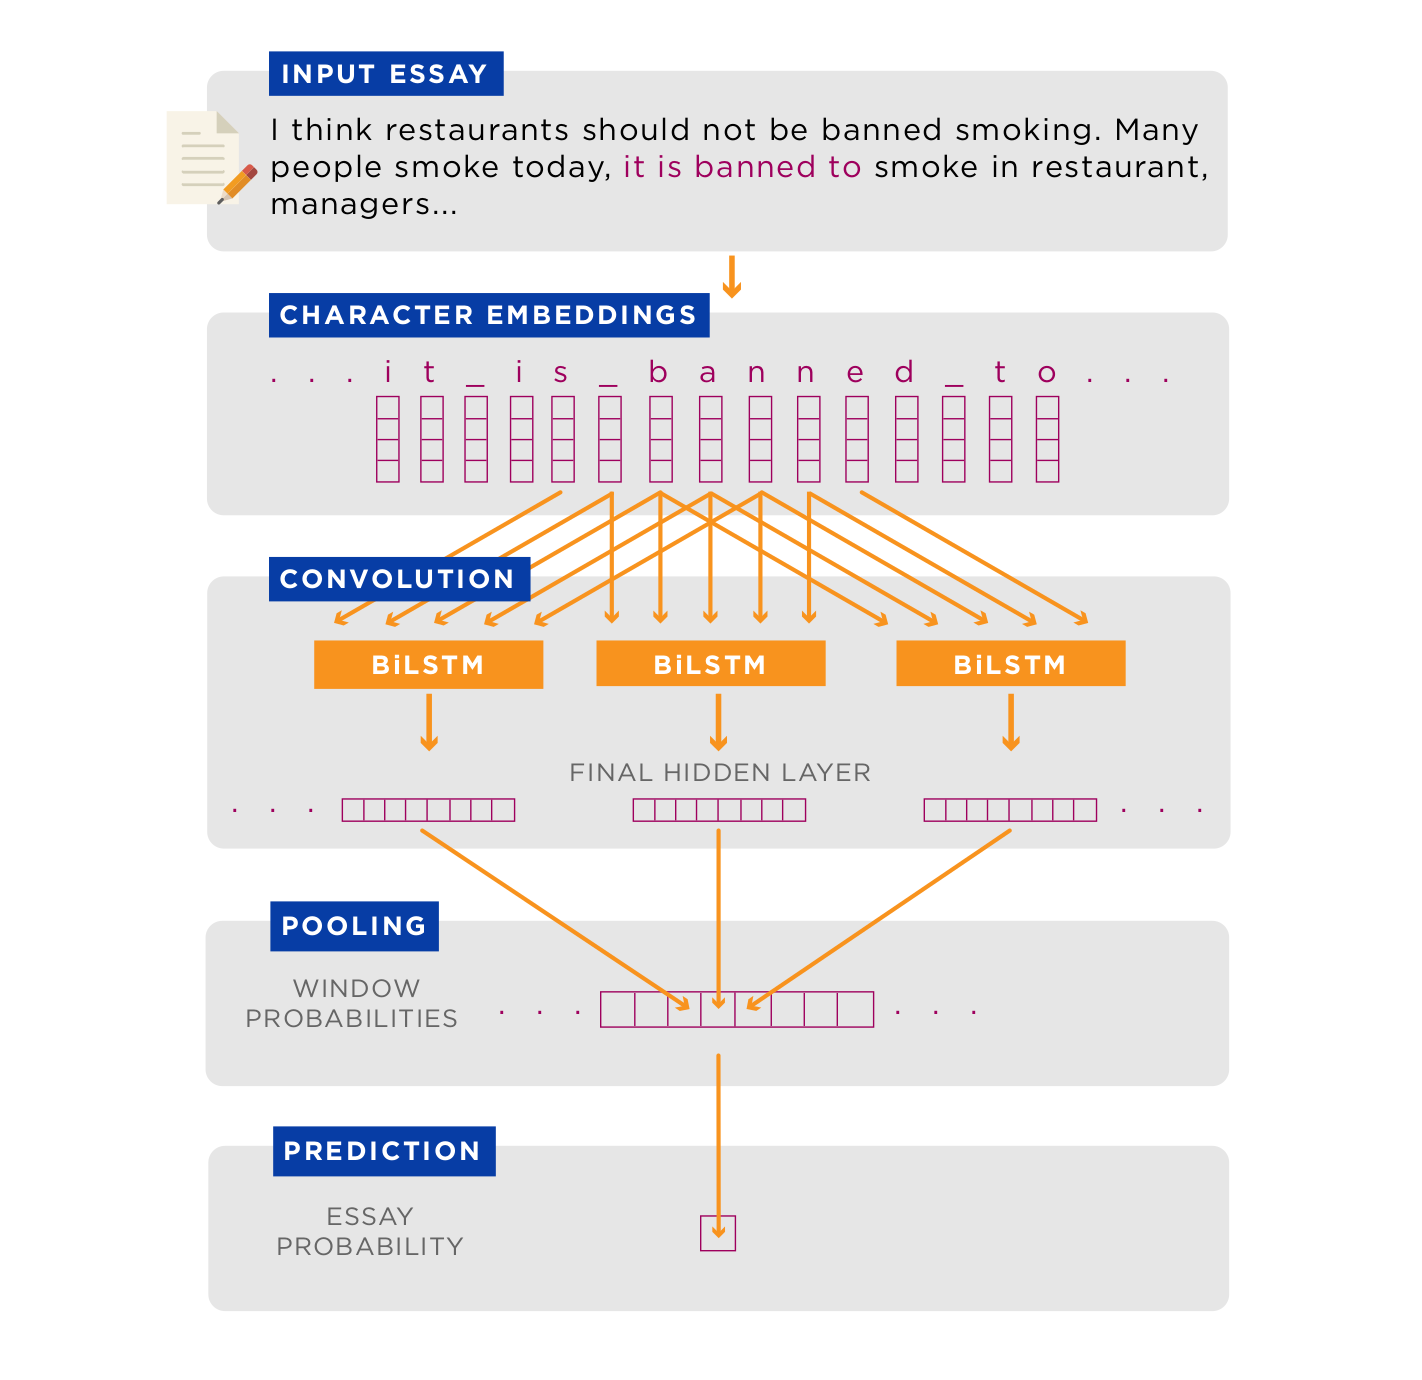
\includegraphics[width=10cm]{deep-filter-pic.png}
\end{center}
\caption{Visualization of the Deep Filter network.} \label{deep-filter-pic}
\end{figure}

The Deep Filter model is the network described above with a deep network
as the convolution. The $f$ function from Equation \ref{log-loss} is a
bidirectional LSTM over character embeddings, with fully connected layer
mapping from the final hidden state of the LSTM to a single text window
probability via a sigmoid activation.

If we represent a standard bidirectional LSTM as
$h_t = BiLSTM(x_1, x_2, \dots, x_t)$, where $x_1, x_2, \dots$ are the elements
of the input sequence and $h_t$ is the concatenation of the final hidden layers
from the forward and backwards LSTMs, then we can write the $f$ function from
Equation \ref{log-loss} as

\begin{equation} \label{final-layer}
f(d_{w_i} = [x_1, x_2, \dots, x_t]) = \sigma (W^{(a)} h_t + b^{(a)})
\end{equation}

Dropout regularization is added between the character embeddings and the LSTM,
as well as between the hidden layer and the affine layer.
Figure \ref{deep-filter-pic} shows the layout of this network.

\subsection{Prompt Aware}


\begin{figure}[h]
\begin{center}
%\framebox[4.0in]{$\;$}
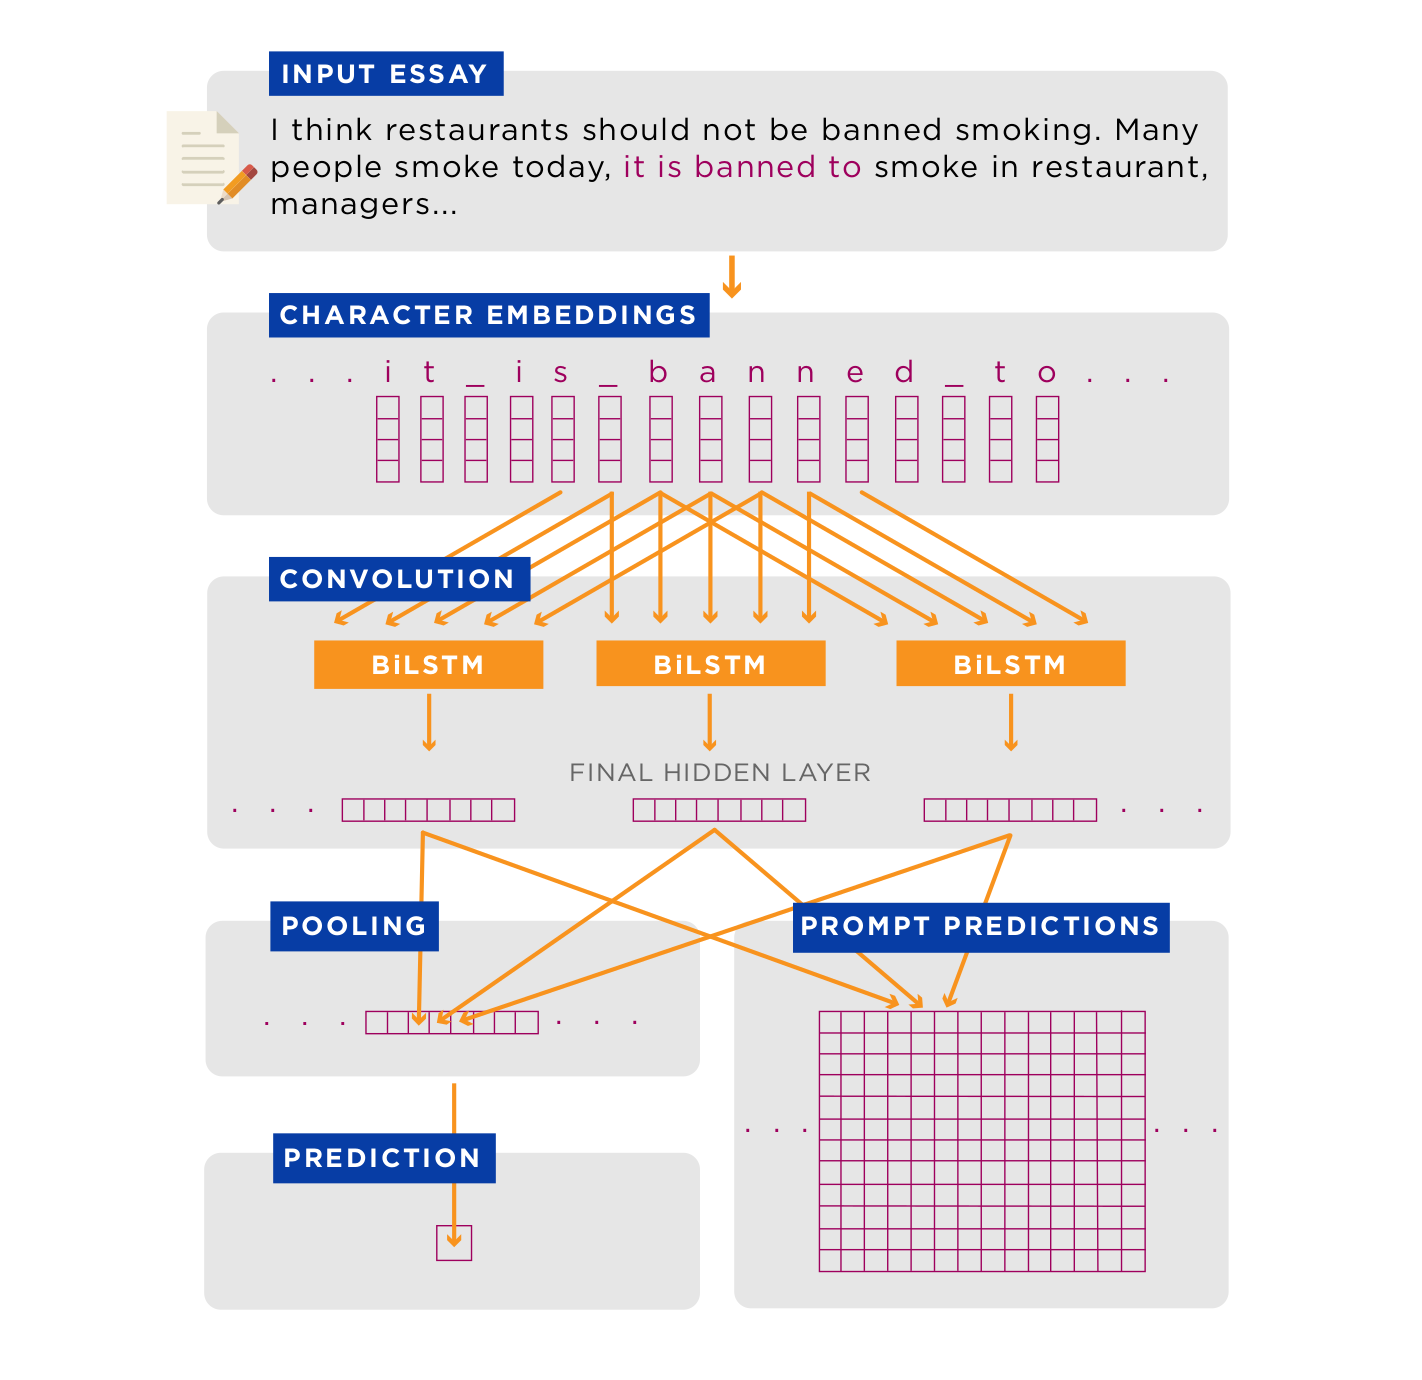
\includegraphics[width=10cm]{prompt-aware-pic.png}
\end{center}
\caption{Visualization of the Prompt Aware network.} \label{prompt-aware-pic}
\end{figure}

One of the potential confounds from the data collection method is that the model
might simply learn the topic of the prompts in each data set. Since the native
English essays in the training and development sets come from different corpora
with different promtps than the ELL essays, this would cause the model to overfit
the training data and show reduced performance on the development and testing sets.
To lessen the effect of this confound, I use a
technique presented by Zhong and Ettinger in \cite{zhong}. They incorporate an
additional module in the network whose objective is to predicit
the confounding factor directly, given the hidden layer as input. The loss from
this prediction is added to the original loss function. By providing the network
with an explicit representation of the confound, it is forced to restrict the space
of possible hypotheses to those that also model the prompt. This acts as a
regularization, allowing the network to generalize better. It is intuitively
similar to regressing out a confound in linear regression.

The Prompt Aware model (Figure \ref{prompt-aware-pic}) uses this idea to extend
the Deep Filter network by adding a module that predicts the prompt each essay
was written to, and adds the loss from this prediction to the existing log loss.
The prediction is the softmax of a fully connected layer that maps the final hidden
layer of the BiLSTM, $h_t$, to a probability distribution over the $n$ prompts
in the training set. At test time, this prediction is ignored.

In order to capture the information about which prompt an essay was written to,
the label that is shown to the network at training time is a tuple
$(y_d, q_d)$. $q_d$ is a one-hot indicator vector, where $q_{d_i}=1$
if the essay $d$ was written to prompt $i$.

Equation \ref{prompt-pred} describes the additional prediction module and
Equation \ref{prompt-loss} gives the updated loss function.

\begin{equation} \label{prompt-pred}
\hat{q} = p(q_d=i | h_t, \theta_q) = softmax(W^{(q)} h_t + b^{(q)})
\end{equation}

\begin{equation} \label{prompt-loss}
L(d, (y_d, q_d)) = -\frac{1}{2}\Big( y_d\, log(c(f(d_{w_{1:k}}))) + (1 - y_d)\, log(1 - (c(f(d_{w_{1:k}})))) \Big) - \frac{1}{2}\sum_{j=1}^k \sum_{z=1}^{|q_d|} q_{d_z} log(\hat{q}_{d_z})
\end{equation}

\section{Experiments} \label{experiments}

Each model is trained to predict the probability that an essay is written by
an ELL student, using information about the student's L1 as the ground truth.
I also hand-annotated $200$ randomly sampled text windows from the test set with
a $1$ if there were errors or awkward phrasing in the window and a $0$ otherwise.
I compare the window predictions from each model (given by the function $f$ in
Equation \ref{log-loss}) to these annotations to see if the model is able to
identify particular subsections of the essay that look incorrect.

As a baseline, I use something like a logistic regression model, in which
the convolutional filter is just a fully connected layer with a sigmoid activation.
The inputs to the baseline network are sparse vectors of character 4-grams per
window of text, where the n-gram index in the feature vector is calculated using
the hashing trick. Instead of dropout, the baseline adds L2 regularization to
the loss.

Table \ref{results-table} shows the area under the ROC curve for all three models
using both max and mean pooling as the pooling layer (function $c$ in Equation
\ref{log-loss}).

Hyperparameters were held constant across all models and were selected for
optimal performance on the development set. Because it takes approximately 3
hours per epoch to train these models, the hyperparamter search was a limited
manual exploration. I have listed the hyperparamter values used in Table
\ref{param-table}. For all models, the development set is evaluated and the
learning rate is scaled down every $20,000$ essays.


\begin{table}[t]
\caption{AUC scores for dev and test}
\label{results-table}
\begin{center}
\begin{tabular}{l r r r}
\multicolumn{1}{l}{\bf MODEL} &\multicolumn{1}{r}{\bf DEV AUC} &\multicolumn{1}{r}{\bf TEST AUC} &\multicolumn{1}{r}{\bf WINDOW AUC}
\\ \hline \\
Logistic Max & 0.711 & 0.569 & 0.583\\
Logistic Avg & 0.771 & 0.796& 0.586\\
Deep Filter Max & 0.787 & 0.693 & 0.591\\
Deep Filter Avg & \textbf{0.922} & \textbf{0.861}  & 0.557\\
Prompt Aware Max & 0.920 & 0.841 & \textbf{0.607}\\
Prompt Aware Avg & 0.917 & 0.856 & 0.597\\
\end{tabular}
\end{center}
\end{table}

\begin{table}[t]
\caption{Hyperparameter values and which models use them}
\label{param-table}
\begin{center}
\begin{tabular}{l c c c c}
\multicolumn{1}{l}{\bf PARAMETER} &\multicolumn{1}{c}{\bf VALUE} &\multicolumn{1}{c}{\bf BASELINE} &\multicolumn{1}{c}{\bf DEEP FILTER} &\multicolumn{1}{c}{\bf PROMPT AWARE}
\\ \hline \\
n epochs & 4 & x & x & x\\
initial learning rate & 0.001 & x & x & x\\
learning rate scaling factor & 0.9 & x & x & x\\
window size (characters) & 100 & x & x & x\\
window stride (characters) & 5 & x & x & x\\
character embedding size & 64 & & x & x\\
LSTM hidden size & 128 & & x & x\\
dropout keep probability & 0.9 & & x & x\\
ngram size (characters) & 4 & x & & \\
feature vector size & $2^{15}$ & x & & \\
L2 regularization lambda & 0.01 & x & & \\
\end{tabular}
\end{center}
\end{table}


\section{Conclusion} \label{conclusion}

\subsection{Analysis} \label{analysis}

Table \ref{results-table} shows that Deep Filter with mean pooling is able to
significantly outperform the baseline on the essay-level classification task.
None of the models show good performance on the window-level task,
although Prompt Aware with max pooling does slightly better than the others.
It is unclear whether the poor performance on the window-level task is due to
the small size of the annotated sample or the fact that the model is picking
up on elements of the writing that indicate the L1 of the author but are unrelated
to the proficiency of the writing. It is interesting to note that mean pooling
outperforms max pooling for the baseline and Deep Filter models, but in the
Prompt Aware model, mean and max pooling are nearly equivalent. More study is needed
to understand why that effect occurs, but it may represent interesting directions
for future research.

Appendix \ref{app-essays} gives examples of the highest and lowest probability
essays according
to the Deep Filter Avg model. Looking at the essay-level predictions on the test
set, it does appear that the essays with a high probability
of being from an ELL writer contain less proficient English writing than those
with low probability. The three prompts are distributed evenly among the high
and low probability essays, and the only noticeable pattern is that high
probability essays tend to have shorter sentences. It is not surprising that
less proficient writers tend to use shorter sentences, so it is hard to tell
from the document level whether this is something the models are picking up on
or if it is simply a correlate.

By loooking at the windows where the model is predicting a high probability,
I am able to infer a little more about what the model is picking up on. Appendix
\ref{app-windows} shows 50 randomly sampled windows where the Prompt Aware Max model
assigned very high or very low probabilities. One thing that jumps out immediately
is that the high probability windows contain
an inordinate amount of transitional phrases. ELL students are often taught to
use standard transitional phrases to enhance the cohesion of their essays.\footnote{
I have learned this from ELL educators that my company has interviewed about the
needs of ELL students.} It is not surprising that low proficiency writers would
tend to lean more heavily on these devices rather than finding varied ways to
keep their essays cohesive. It also makes sense that the model might pick up on
this easy indicator of ELL writing.

The high probability windows without transitional
phrases also show evidence of low-proficiency writing, mostly due to
grammatical issues. It may be interesting to try to control for the effect of
transitional phrases in future work.


\subsection{Next steps} \label{future}

There are a number of things about this study that could be improved upon in
future work. First and foremost, it would be useful to have a data set with
labels directly related to the proficiency of the essays or the individual sentences,
rather than trying to infer that information using the L1 of the author as a proxy.

I believe that the high performance of the classifier on data sets and prompts
that were unobserved during training indicates that the model is not picking up
on prompt-specific language, but to be sure, it would be nice to collect a large
data set of native and non-native English writers all responding to the same
prompt under the same controlled circumstances.

The advantage of the method used in this paper is that the native/non-native label
is very easy to obtain. It may be possible to achieve better results by adding a
a lot more native English writing, and using a langugage model trained on the
native English writing to find areas of low proficiency based on high perplexity
sections of the text.



\begin{thebibliography}{6}

\bibitem{chollampatt}
    Chollampatt, Shamil, Kaveh Taghipour, and Hwee Tou Ng.
    "Neural network translation models for grammatical error correction."
    \emph{arXiv preprint} arXiv:1606.00189 (2016).

\bibitem{liu}
    Liu, Zhuoran, and Yang Liu.
    "Exploiting Unlabeled Data for Neural Grammatical Error Detection."
    \emph{arXiv preprint} arXiv:1611.08987 (2016).

\bibitem{bryant}
    Bryant, Christopher, and Hwee Tou Ng.
    "How Far are We from Fully Automatic High Quality Grammatical Error Correction?."
    \emph{ACL} (1). 2015.

\bibitem{tomokiyo}
    Tomokiyo, Laura Mayfield, and Rosie Jones.
    "You're not from 'round here, are you?: naive Bayes detection of non-native utterance text."
    {Proceedings of the second meeting of the North American Chapter of the Association
    for Computational Linguistics on Language technologies.} Association for Computational Linguistics, 2001.

\bibitem{malmasi}
    Malmasi, Shervin, Joel Tetreault, and Mark Dras.
    "Oracle and human baselines for native language identification."
    \emph{Proceedings of the Tenth Workshop on Innovative Use of NLP for Building
    Educational Applications.} 2015.

\bibitem{goutte}
    Goutte, Cyril, et al.
    "Discriminating similar languages: Evaluations and explorations."
    \emph{arXiv preprint arXiv:1610.00031} (2016).

\bibitem{baroni}
    Baroni, Marco, and Silvia Bernardini.
    "A new approach to the study of translationese: Machine-learning the difference
    between original and translated text."
    \emph{Literary and Linguistic Computing} 21.3 (2006): 259-274.

\bibitem{tang}
    Tang, Duyu, Bing Qin, and Ting Liu.
    "Document Modeling with Gated Recurrent Neural Network for Sentiment Classification."
    \emph{EMNLP}. 2015.

\bibitem{yang}
    Yang, Zichao, et al.
    "Hierarchical attention networks for document classification."
    \emph{Proceedings of NAACL-HLT}. 2016.

\bibitem{mikolov}
    Le, Quoc V., and Tomas Mikolov.
    "Distributed Representations of Sentences and Documents."
    \emph{ICML}. Vol. 14. 2014.

\bibitem{collobert}
    Collobert, Ronan, et al.
    "Natural language processing (almost) from scratch."
    \emph{Journal of Machine Learning Research} 12.Aug (2011): 2493-2537.

\bibitem{zhong}
    Zhong, Yu, and Gil Ettinger.
    "Enlightening Deep Neural Networks with Knowledge of Confounding Factors."
    \emph{arXiv preprint arXiv:1607.02397} (2016).
\end{thebibliography}

\clearpage

\appendix

\section{Data} \label{app-data}

\begin{table}[H]
\caption{ELL and Native English Corpora}
\label{data-table}
\begin{center}
\begin{tabularx}{\textwidth}{l r r X}
\multicolumn{1}{c}{\bf CORPUS} &\multicolumn{1}{c}{\bf $n$ ESSAYS} &\multicolumn{1}{c}{\bf $n$ PROMPTS} &\multicolumn{1}{c}{\bf L1s}
\\ \hline \\
\hline
\href{http://language.sakura.ne.jp/icnale/}{ICNALE} & $5,600$ & $2$ & CHN, \textbf{ENG}, FIL, HKG, IND, JPN, \newline KOR, PAK, SIN, THA, TWN \\
\href{http://www.comp.nus.edu.sg/~nlp/conll14st.html\#nucle32}{NUCLE} & $1,397$ & $3$ & CHN \\
\href{http://ilexir.co.uk/datasets/index.html}{FCE} & $2,481$ & $44$ & CAT, CHN, FRA, GER, GRC, ITA, \newline JPN, KOR, NL, POL, PRT, RUS, \newline SPA, SWE, THA, TUR \\
\href{https://meta-toolkit.org/data/2016-01-26/ceeaus.tar.gz}{CEEAUS} & $1,008$ & $2$ & CHN, \textbf{ENG}, JPN \\
\href{http://www.u-sacred-heart.ac.jp/okugiri/links/moecs/links/data/data.html}{MOECS} & $199$ & $1$ & \textbf{ENG}, JPN \\
\href{http://koreanlearnercorpusblog.blogspot.be/p/corpus.html}{Gachon} & $15,831$ & $20$ & KOR \\
\href{http://www.bfsu-corpus.org/static/corpora/TECCL_Corpus_V1.1.zip}{TECCL} & $9,864$ & $???$ & CHN \\
Private A & $550$ & $1$ & KOR \\
Private B & $4,694$ & $4$ & CHN \\
\href{https://catalog.ldc.upenn.edu/LDC2014T06}{TOEFL-11} & $12,100$ & $8$ & ARA, CHN, FRA, GER, IND, ITA, \newline JPN, KOR, SPA, TEL, TUR \\
Private C & $41,227$ & $53$ & \textbf{ENG} \\
Private D & $29,559$ & $21$ & \textbf{ENG} \\
\href{https://www.kaggle.com/c/asap-aes/data}{ASAP} & $17,677$ & $8$ & \textbf{ENG} \\
\end{tabularx}
\end{center}
\end{table}

\begin{table}[H]
\caption{L1s}
\label{L1s-table}
\begin{center}
\begin{tabularx}{\textwidth}{l l l l l l }
\multicolumn{1}{c}{\bf ABBREVIATION} & \multicolumn{1}{c}{\bf LANGUAGE} \\
\hline
ARA & Arabic &    GRC  & Greek   &          PRT  & Portuguese \\
BUL & Bulgarian &      HKG  &  Hong Kong Cantonese       &    RUS  & Russian \\
CAT & Catalan &    IND  & Indian languages   &           SIN  & Singapore languages \\
CHN & Chinese &    ITA  & Italian        &   SPA  & Spanish \\
CZE & Czech &     JPN  & Japanese         &     SWE  & Swedish \\
ENG & English &    KOR  & Korean         &   TEL  & Telugu \\
FIL & Filipino &       NL  &  Dutch      &       THA &  Thai \\
FIN & Finnish &    NOR &  Norwegian       &      TSW  & Tswana \\
FRA & French &     PAK  & Urdu         &     TUR  & Turkish \\
GER & German &     POL  & Polish    &        TWN  & Taiwanese
\end{tabularx}
\end{center}
\end{table}


\begin{table}[H]
\caption{Further info for each public subcorpus}
\label{further-info}
\begin{center}
\begin{tabular}{r l}
ICNALE & http://language.sakura.ne.jp/icnale/ \\
NUCLE & http://www.comp.nus.edu.sg/~nlp/conll14st.html\#nucle32 \\
FCE & http://ilexir.co.uk/datasets/index.html \\
CEEAUS & https://meta-toolkit.org/data/2016-01-26/ceeaus.tar.gz \\
MOECS & http://www.u-sacred-heart.ac.jp/okugiri/links/moecs/links/data/data.html \\
Gachon & http://koreanlearnercorpusblog.blogspot.be/p/corpus.html \\
TECCL & http://www.bfsu-corpus.org/static/corpora/TECCL\_Corpus\_V1.1.zip \\
TOEFL-11 & https://catalog.ldc.upenn.edu/LDC2014T06 \\
ASAP & https://www.kaggle.com/c/asap-aes/data
\end{tabular}
\end{center}
\end{table}

\clearpage
\section{Essays} \label{app-essays}

\textbf{Highest probability of being an ELL writer, according to Deep Filter Avg}
\begin{displayquote}
Time is Internet Now, all over the world, we can use Internet freely. Someone
says newspaper and magazine are not useful, because we can take news by
Internet, the other says newspaper and magazine are necessary. In my opinion,
newspaper and magazine are not necessary. I have two opinions. Firstly, It is
easy to take news everywhere by Internet. Secondly, we can get world news.
Internet has many information, but newspaper is limitted. When we want
information, we can for it by Internet. However, someone says it is important
to read words. When we use Internet, we watch only interested news, but we
don't pay attention to newspaper and magazine, we catch news by eyes. But, now,
time is Internet world. We have computer necessary. We can see newspaper by
Internet. Company of newspaper keeps up with time. There are many bad
information in Internet, so we should judge good or bad. We are required skill
of judgement. If we use Internet correctly, Internet would be best way that we
get news. That is why nowadays newspaper and magazine are not more and more
useful.
\end{displayquote}

\textbf{Lowest probability of being an ELL writer, according to Deep Filter Avg}
\begin{displayquote}
I don't agree because I think that this is more to do with being a private,
informal arrangement between restaurant owners and people who patronise their
restaurants. The owners either allow smoking on the premises or they do not.
If patrons find a smoking restaurant offensive then it is a simple decision
not to go to smoking restaurants. I am not sure if the Japanese Government
has a say in this side of things under Japanese law and I am not a lawyer.
Like most governments though, I suppose that they could either re-write or
override and laws really since they are the government. I don't smoke but I
have friends that do and they are usually quite considerate about where they
blow their smoke. Not that I am making excuses and I neither condemn them or
condone their smoking because it is their lives after all and provided they do
not infringe on mine or anyone else's health than I guess that they are free
to do as they like. So long as they are obeying the local laws of the land
wherever they may happen to reside than I think that it is a case of live and
let live.
\end{displayquote}
\clearpage
\section{Windows} \label{app-windows}
\textbf{Windows where Prompt Aware Max predicted $p = 1.0$}

\texttt{\fontsize{.28cm}{.1cm}\selectfont \frenchspacing . For example, I have more opportunities to have dinner with friends and to go shopping. And if we e}
\texttt{\fontsize{.28cm}{.1cm}\selectfont \frenchspacing income but I think that part time job is only suitable for student who can learn very well. Because }
\texttt{\fontsize{.28cm}{.1cm}\selectfont \frenchspacing lace a student-employee ahead of the curve when they enter the full-time workforce. And than, Experi}
\texttt{\fontsize{.28cm}{.1cm}\selectfont \frenchspacing nd more part-time jobs turn up.And the jobs have enormous attraction to college students. As a resul}
\texttt{\fontsize{.28cm}{.1cm}\selectfont \frenchspacing nd three positive points about using the Internet. First, you can get the information very quickly. }
\texttt{\fontsize{.28cm}{.1cm}\selectfont \frenchspacing ct yourself is a thing we should learn. At last, part time job is a first step for your working life}
\texttt{\fontsize{.28cm}{.1cm}\selectfont \frenchspacing ough smoking is not welcomed in public places, we can make it too strict. However, we can set some r}
\texttt{\fontsize{.28cm}{.1cm}\selectfont \frenchspacing  are three reasons I think so. By the way I have a part-time job. I wrote reasons which base on my e}
\texttt{\fontsize{.28cm}{.1cm}\selectfont \frenchspacing know that they do themselves harm and give trouble to a lot of people. Finally, I think they should }
\texttt{\fontsize{.28cm}{.1cm}\selectfont \frenchspacing arette. We became unwillingly second-hand smokers. This is happening to me very often and every time}
\texttt{\fontsize{.28cm}{.1cm}\selectfont \frenchspacing . Finally, to work somewhere is good experience. Not only college students but also high school stud}
\texttt{\fontsize{.28cm}{.1cm}\selectfont \frenchspacing nd easily a part-time job for student anywhere. A part-time job contributes to many an advantage for}
\texttt{\fontsize{.28cm}{.1cm}\selectfont \frenchspacing ink it is important for college students to have a part-time job.There are some reasons I think so.F}
\texttt{\fontsize{.28cm}{.1cm}\selectfont \frenchspacing make eyes and throat sore. Smoke will bother people who want to enjoy and relax their time at the re}
\texttt{\fontsize{.28cm}{.1cm}\selectfont \frenchspacing mples. We know people in the restaurants all want to be healthy. On the other hand, smoking in the r}
\texttt{\fontsize{.28cm}{.1cm}\selectfont \frenchspacing their college life are important. In my opinions, first, most of students don't have to leave their }
\texttt{\fontsize{.28cm}{.1cm}\selectfont \frenchspacing hich is related English. As these reason, I think it is important for college students to have a par}
\texttt{\fontsize{.28cm}{.1cm}\selectfont \frenchspacing ocial life. However, I believe that degree is not an identification of successfulness. This essay ai}
\texttt{\fontsize{.28cm}{.1cm}\selectfont \frenchspacing own gradually and the color of the wall makes the restraint's impression bad. Managers have to pay m}
\texttt{\fontsize{.28cm}{.1cm}\selectfont \frenchspacing They didn't know the application of the theory. In conclusion, have a part time job is very importan}
\texttt{\fontsize{.28cm}{.1cm}\selectfont \frenchspacing  world rely on and use the internet to access information such as the news, newspapers and magazines}
\texttt{\fontsize{.28cm}{.1cm}\selectfont \frenchspacing  at the university. Nowadays, many students have a part time job. I think that it could be important}
\texttt{\fontsize{.28cm}{.1cm}\selectfont \frenchspacing for your studying branch, it can give you more practical knowledge of your studying, enhances your k}
\texttt{\fontsize{.28cm}{.1cm}\selectfont \frenchspacing llege students to have a part-time job. It makes extra income during study. It is training a good ex}
\texttt{\fontsize{.28cm}{.1cm}\selectfont \frenchspacing  society. Second reason, it is good for college students economically. Many college students need mu}
\texttt{\fontsize{.28cm}{.1cm}\selectfont \frenchspacing ampus is no longer that peaceful because so many students are engaged in their job. But please remem}


\textbf{Windows where Prompt Aware Max predicted $p \le 3.5 \times 10^{-10}$}

\texttt{\fontsize{.28cm}{.1cm}\selectfont \frenchspacing to these smokers could probably cause them to have an asthma attack and end up lying on a hospital b}
\texttt{\fontsize{.28cm}{.1cm}\selectfont \frenchspacing t our children even if they are not anymore kids. Not like kids in the US, that when out of High Sch}
\texttt{\fontsize{.28cm}{.1cm}\selectfont \frenchspacing  Government would be taking away a person's or restaurant's choice and then what are they left with?}
\texttt{\fontsize{.28cm}{.1cm}\selectfont \frenchspacing ion that in the case of drugs, there are a number of drugs that have no long-lasting ill-effects on }
\texttt{\fontsize{.28cm}{.1cm}\selectfont \frenchspacing t has it ever come to your ind that there are also other people around you? Smoking may be just for }
\texttt{\fontsize{.28cm}{.1cm}\selectfont \frenchspacing these systems randomly and spontaneously shutdown? How would anyone be able to read about the news i}
\texttt{\fontsize{.28cm}{.1cm}\selectfont \frenchspacing because it offers them chances to practice what they have learnt in school and learn something beyon}
\texttt{\fontsize{.28cm}{.1cm}\selectfont \frenchspacing rettes because there is no air ventilate to get rid of all smoke but it will be in their breath and }
\texttt{\fontsize{.28cm}{.1cm}\selectfont \frenchspacing em because they can get all smoke into their body and smoke can cause lots of disease such as cancer}
\texttt{\fontsize{.28cm}{.1cm}\selectfont \frenchspacing y anything you want but you should limit yourself. As we all know that it can be a distraction to th}
\texttt{\fontsize{.28cm}{.1cm}\selectfont \frenchspacing es. Since you will eventually have to pay off any school-related loans that you take out, it is best}
\texttt{\fontsize{.28cm}{.1cm}\selectfont \frenchspacing anging from news articles to videos all available online. This has lead to a debate regarding the ne}
\texttt{\fontsize{.28cm}{.1cm}\selectfont \frenchspacing they couldn't handle with the scholar task and others just for having some extra pocket money. In th}
\texttt{\fontsize{.28cm}{.1cm}\selectfont \frenchspacing d 6 million people may die each year worldwide because of tobacco smoking and diseases related to it}
\texttt{\fontsize{.28cm}{.1cm}\selectfont \frenchspacing ins and bus have a seat that can't use cell phone here!! Please turn off your cell phone and each of}
\texttt{\fontsize{.28cm}{.1cm}\selectfont \frenchspacing taurant they desire without having to worry about being exposed to secondhand smoke that could cause}
\texttt{\fontsize{.28cm}{.1cm}\selectfont \frenchspacing ous. We should ask our kids to keep far away from smoking, and make posters or videos to make people}
\texttt{\fontsize{.28cm}{.1cm}\selectfont \frenchspacing f printed material and distribute it distances that our ancestors would not be able to believe, on a}
\texttt{\fontsize{.28cm}{.1cm}\selectfont \frenchspacing l have the responsibly of getting to work on time, being organized with their uniforms etc. Being in}
\texttt{\fontsize{.28cm}{.1cm}\selectfont \frenchspacing rs if they are helping you with your expenses. Your parents will not be around forever, and so you h}
\texttt{\fontsize{.28cm}{.1cm}\selectfont \frenchspacing rettes. As you can see, if your smoking it Impact to you are family or people you are love and your }
\texttt{\fontsize{.28cm}{.1cm}\selectfont \frenchspacing r to everyone, this way everyone would be happy because the smokers would get to smoke whenever they}
\texttt{\fontsize{.28cm}{.1cm}\selectfont \frenchspacing ery through from them to through that addiction away. Some people smoke only for joy or seeing someo}
\texttt{\fontsize{.28cm}{.1cm}\selectfont \frenchspacing ple to smoke in. That way they could still smoke but bystanders wouldn't need to be exposed to it. I}
\texttt{\fontsize{.28cm}{.1cm}\selectfont \frenchspacing  issues from different ways that will help you learn a skill that you needed to but couldn't previou}
\texttt{\fontsize{.28cm}{.1cm}\selectfont \frenchspacing ir and make an annoyed to people around not just annoying but it can make pollution spread into the }


\end{document}
